\documentclass{standalone}
\usepackage{tikz,amsmath,amssymb}

\begin{document}
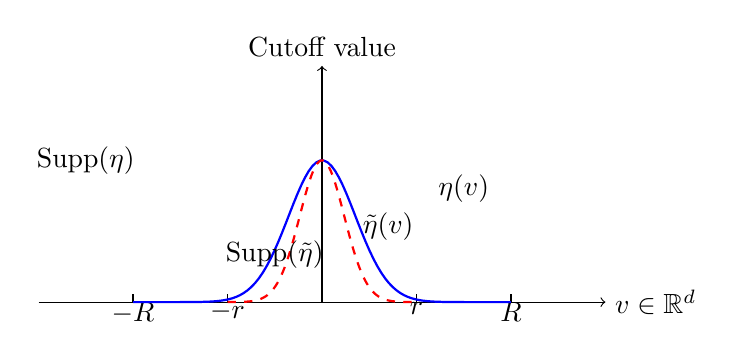
\begin{tikzpicture}[scale=1.2]
  % Axes
  \draw[->] (-3,0) -- (3,0) node[right] {$v \in \mathbb{R}^d$};
  \draw[->] (0,0) -- (0,2.5) node[above] {Cutoff value};
  
  % Support markers
  \draw[dashed] (-2,0) -- (-2,0.1) node[below] {$-R$};
  \draw[dashed] (2,0) -- (2,0.1) node[below] {$R$};
  \draw[dashed] (-1,0) -- (-1,0.1) node[below] {$-r$};
  \draw[dashed] (1,0) -- (1,0.1) node[below] {$r$};
  
  % Cutoff eta (blue solid)
  \draw[thick, blue, domain=-2:2, samples=100] 
    plot (\x, {1.5*exp(-4*(\x)^2)});
  
  \node at (1.5,1.2) {$\eta(v)$};
  
  % Cutoff tilde eta (red dashed)
  \draw[thick, red, dashed, domain=-1:1, samples=100] 
    plot (\x, {1.5*exp(-9*(\x)^2)});
  \node at (0.7,0.8) {$\tilde{\eta}(v)$};
  
  % Annotations
  \node at (-2.5,1.5) {$\text{Supp}(\eta)$};
  \node at (-0.5,0.5) {$\text{Supp}(\tilde{\eta})$};
\end{tikzpicture}
\end{document}